\documentclass[openany]{article}
\usepackage[T1]{fontenc}
\usepackage[utf8]{inputenc}
%\usepackage[icelandic]{babel}
\usepackage{caption}
\usepackage{circuitikz}
\usepackage{grffile} 
\usepackage[margin=1in]{geometry}
\usepackage[icelandic]{babel}
\usepackage{listings}

% grffile er pakki sem leifir manni að nota "" til þess að forðast að nota
% nafnið á myndinni með.
\usepackage{graphicx}
% \graphicspath{{images/}} Sýnir undir möppu þar sem myndirnar eru

\usepackage{hyperref}
%fyrirlinka - \url{www.....}
\begin{document}


\title{Þróunhugbúnaðar \\
Lokaprófs undirbúningur}
\author{Pétur}
\maketitle

\pagebreak

\tableofcontents

\pagebreak

\section{Software Engineer}
\subsection{Definition}
Hugbúnaðarverkfræðingur verður að hafa góð tök á forritun, slunginn í reikniritum og uppbyggingu gagna. Verkfræðingurinn þarf að hafa góð skil á nokkrum hönnunar módelum heldur en að geta forritað þau.
\subsection{Important skills}
\begin{itemize}
	\item Góða samskiftar hæfileika
	\item Getað búið til líkön af flóknum verkefnum
	\item Getað skipulagt og stjórnað vinnu
\end{itemize}
\section{General project work}
\subsection{Reasons for failure}
\subsubsection{Excessive schedule}
Ef það er of mikið vinnuálag á verkefninu sem unnið er að þá getur verkefnið átt í hættu að vera unnið illa.
\subsubsection{Changing needs}
Breytingar í miðju verkefni geta haft slæm áhrif á verkefni sem unnið er að.
\subsubsection{Lack of documented project plan}
Mikilvægt er að hafa allt nánast ritað í stein svo vinnu menn geta verið á sömublaðsíðu.
\subsection{Causes of Software Project Troubles}
\begin{itemize}
	\item Verkefni unnið í nýju software umhverfi
	\item Breyting á viðskiptavinum 
	\item Tími sem fer í að læra á verkefnið
	\item Miskilningur, mismunandi markmið og uppgjöf á verkefni.
\end{itemize}
\section{Software Process Models}
\subsection{Big Bang Approach}
Hönnuður fær engar athugasemdir frá kúnna
\subsection{The Waterfall Model}
Hönnuður fær athugasemdir frá kúnna og þarf að endurtaka sum hönnunarskref aftur.
\subsection{Plan-driven}
Skipulags módel reynir að komast að öllu í byrjun og heldur sig við ákvarðanir.
\begin{itemize}
	\item Reyna að skilja og plana fyrir fram stóra hluti af verkefninu og skilgreina það ítarlega í byrjun verkefnis
	\item Skipt er verkefni niður á hönnuði
	\item Föst skilar áætlun fyrir hvern þátt í verkefninu
	\item Lítið rými fyrir breytingar á verkefni þegar það er komið í mitt kaf
	\item Mikinn skilning og yfir sýn á framþróun útkomu verkefnisins
	\item Spíral módel ...
\end{itemize}
\subsection{Agile Models}
Sveigjanleg módel Skrifa og endurgera planið fyrir næstu ítranir meðan verkefninu stendur yfir.
\begin{itemize}
	\item Byrja með hráa mynd af verkefni, fínpússa sig í gegnum margar prótótýpur og lykkjur af athugasemdum frá viðskiptavini
	\item Hönnuður(developer) fær að velja sér verkefni
	\item Skil á þáttum(component) er hægt að enduskipuleggja skilar tíma og mikilvægi hvenær sem er.
	\item Engar skilgreind atriði og plön
	\item Lítil stjórnun, yfirsín yfir hvernig verkefnið gengur og mun vera.
\end{itemize}

\section{Software Engineer}
\subsection{Definition}
Hugbúnaðarverkfræðingur verður að hafa góð tök á forritun, slunginn í reikniritum og uppbyggingu gagna. Verkfræðingurinn þarf að hafa góð skil á nokkrum hönnunar módelum heldur en að geta forritað þau.
\subsection{Important skills}
\begin{itemize}
	\item Góða samskiftar hæfileikar.
	\item Getað búið til líkön af flóknum verkefnum
	\item Getað skipulagt og stjórnað vinnu.
\end{itemize}

\section{Requirements Engineering}
\subsection{Functional requirement}
Skilgreina eiginleikar sem hugbúnaðurinn verður að hafa. \textbf{Dæmi}: Ökumaður verður látin vita ef þrýstingur í dekkjum er lár.
\subsection{Quality requirement}
Skilgreina þægindinn á bakvið búnaðinn. \textbf{Dæmi}: Leit í leitarvélin tekur í mestalagi 1 sekúndu.
\subsection{General condition}
Almennt sem má búast af vörunni. \textbf{Dæmi} appið sem er verið er að þróa þarf að líta snirtilega út.
\subsection{Conflicts}
\subsubsection{Subject conflict}
Misskilið eða vitlausar upplýsingar, mismunandi túlkun staðreynda.
\subsubsection{Conflict of interest}
Mismunandi áhugi, mismunandi áætlanir og markmið fjárfesta.
\subsubsection{Value conflict}
Mismunandi skoðanir tengdir ákveðnum hlutum. Til dæmis menningarlegir mismunir.
\subsubsection{Structural conflict}
Ójafnvægi í valdadreifingu.
\subsubsection{Imagine the university contracted you to build a new social networking site for all students. Explain two types of conflicts that you may run into during the requirements elicitation and give an example for each of them}
Subject conflict ef þeir gefa mér verkefnið og ég skil ekki upplýsingarnar sem mér voru gefnar til þess að gera tengsla netsíðuna þá getur átt sér stað deila um hvernig niðurstaðan á að vera. Conflict of interest ef ég sem hönnunður er að vinna í síðunni vill leggja mikla áherslu á að útfæra einnhvað x sem ég held að væri gott fyrir vefinn. En kúninn hefur allt aðra áherslu og vill útfæra b þá getur mindast deila milli míns og kúnnans.
\subsection{Technical detail in user story}
\subsubsection{User story recipe}
\textbf{ \{ Role/Perspective, Goal/Function, Rational/Benefit(optional)\}}
\begin{itemize}
	\item Role/Perspective: Sem notandi
	\item Goal/Function: Ég vill getað leitað af hótelum með fillterum
	\item Rational/Benefit(optional): , svo að ég get fundið hótelið sem ég vill bóka
\end{itemize}
\subsubsection{How much technical detail should be in a user story}
Í notendar sögu þá ætti ekkert af tæknilegum atriðum, lausnum að koma framm. Ef tæknilegu atriðin koma fram þá þarf kúnninn að geta skilið þau líka. Kúninn og ég við þurfum að geta skilið notendasögurnar.
\subsubsection{Example: good user story}
\textit{Bókun flugs}: Notandi verður að geta bókað flug á ákveðnum tíma og dagsetningu.
\subsubsection{Example: bad user story}
\textbf{Nota jflex fyrir UI}: Notendar viðmótið mun nota jflex til þess að sýna gögninn á flottan máta.
\section{Effort Estimation}
Leið til þess að ákvaða hversu mikinn tíma þarf til þess að setja í hver verk.
\subsection{Planing poker}
Planing poker er þannig að hver meðlimur hóps fær 13 spil sem hafa mismunandi daga fjölda til þess að geta metið hvað hvert verkefni taki langan tíma. Einn hringur er þannig að verkefni er lagt á borð svo velja allir eitt spil í leind og sína svo allir spilin sín og ræða niðursöðurnar sínar. Í sameiningu þá er tekið ákvörðun útfrá röksæmdarfærslu annara, hverssu mikinn tíma hópurinn heldur í raun og veru hverssu mikinn tíma fer í verkið.
\subsubsection{Based on differing skills and experience, individual team members may estimate different efforts for any requirement. Discuss whether planning poker eliminates this problem}
Ef það kemur upp að hópur af fólki sem er að spila planing poker og er með breytilegt getustig. Þá er hættan að fólk mun kjósa mjög breytilega. Það er samt gott því þá opnar það fyrir umræðuna afhverju eru svörin svona breytileg. Það getur reynst að fólki finnist verkið svo flókið fyrir sig að það kýs rosalega háa tölu. Sama fyrir fólkið sem finnst þetta rosalega létt sem mun kjósa þá lágu töluna. Með þessa niðurstöður þá getur fólkið sem hefur gert þennan verkþátt áður og veit betur en fólkið sem kaus mjög hátt fyrir verkþáttin. Sagt þeim ástæðuna afhverju þau kusu svona lágt og hvernig verkefnið verður leist. Þar með sannfært fólkið með minni kunnátuna að breyta um skoðun og færast nær sinni skoðun. Þetta getur virkað einnig í hina áttina. Fólkið sem heldur að þetta er auðvellt en í raun og veru þá sá fólkið sem kaus háatölu vandarmál sem væri erfitt að leisa. Það segir fólkinu sem kaus lágt frá þessu vandarmáli og fær það til þess að kjósa nær sér í tölu. Planing poker mun leisa þetta vandarmál að vissuleiti því planing poker er góð leið til þess að vekja upp umræður fólks á verkefninu sem mun vera unnið að.
\subsubsection{Assume your team came up with an effort spread of 8, 13, 40 and 40 for a particular user story. Interpret and deal with the result}
Gefum okkur að það var kosið fyrir notenda sögu x. þar sem það var kosið 8, 13, 40 og 40 þá er líklega misræmi í getustigi. Þeir sem kusu minnst þá 8 þarf 
að útskíra fyrir hinum afhverju hann haldi að útfæra þessa notendasögu muni vera svona létt. 13 mun vera skilningsríkar á því afhverju 8 kaus 8. En svo er það að 8 og 13 þurfa líkleg ræða mikið við 40 og 40 afhverju þarna er svona mikill munur. Það er hugsanlegt að það er mikill munur á getustigi, að báðar 40 vita ekki neitt hvernig á að útfæra notendarsöguna eða að þær sjá stæri vanda sem 8 og 13 sjá ekki. Svo getur þetta virkað á hinn bógin líka að af því að 8 og 13 kunna að gera verkefnið og báðar 40 sjá fram á það að þurfa að læra mikið til þess að geta unnið verkið. Það getur líka reynst að 8, 13 sjá strax lausnina en báðar 40 sjá hana ekki en þegar 8 og 13 hjálpa til við að útskíra lausnina þá sjá 40 og þá munu þeir vera á sömublaðsíðu.


\subsection{Anchoring effect}
Ef þú ert með tölu í hausnum á þér þá mun hún hafa áhrif á matið þitt. Jafnvel ef þú ert sérfræðingur á sviðinu. Dæmi: Hvað varð Ghandi 144 ára gamall. Þá er manneskjan svö föst á tölunni og mun giska í kringum hana.

\section{Project Planning}
\subsection{Calculating new velocity}
Byrjunar hraði er stundum metinn þannig að valið er 0.7 sem er dæmigerður verktími fyrir hugbúnaðargerð. Einnig er hægt að velja hraða úr fyrri verkefnum. Nýr vinnu hraði er alltaf endur reiknaður eftir hvern áfanga til þess að fá raunhæfa sýn yfir vinnu getu hópsins. Dæmi um reikning á vinnu hraða:
\begin{itemize}
	\item Summa saman persónu daga úr verkefninu sem klárað var
	\item Deila því með persónu dögunum
	\item Hef 20 vinnu daga, 3 vinnendur, kláruð verk 38 persónu dagar
	\item $\frac{KlarudVerkIPersonuDogum}{vinnendur * vinnudaga}$
	\item Hraðinn er: $\frac{38}{3 * 20} = 0.6$ 
\end{itemize}
\subsection{Predicting how much you can get done next time}
Með nýja hraðanum er hægt að meta hverssu mikið það er hægt að áorka í næsta þætti. Dæmi:
\begin{itemize}
	\item Næsti þáttur er 1 mánuður 20 dagar
	\item Þrír sem ætla að vinna að verkinu
	\item þannig tími sem er metinn í að hverssu mikið verður klárað þann mánuð er
	\item Þannig að í næsta þætti þá mun aðeins ná að klára svon marga vinnu daga $60 * 0.6 = 36$
\end{itemize}
\subsection{Assume your 4-person team completed tasks comprising 20 person-days in a 2-week iteration. Calculate the velocity you should assume when planning the next iteration}
Tvær vikur þá hef ég tíu vinnudaga sem unnið var. þannig að þá er hraðinn $\frac{20}{4*10} = 0.5$
\subsection{Imagine the a client expects more functionality in a release then you will be able to complete until the deadline, based on your effort estimates. Suggest a strategy you could use in this situation}
Með höndla nýja verkefnið eins og önnur, skoða verkefnið og fá á hreinnt hvað gera skal. Brjóta verkefnið upp ef þess þörf er á. Meta og forgangsraða bæta svo við burn down chart. Það er hægt að semja við kúnna að það þurfi að færa verkefni yfir á næsta þátt eða sleppa hluta verkefnis til þess að koma því nýja inn.

\section{Object-Oriented Analysis and Design}
\subsection{Associations}
Tenging opin örvar oddur [class|car] -wheels -> [class|wheel] Sem sýnir að bíll hefur tengingu við dekk, bíll þarf dekk til þess að keyra.
\subsection{Aggregation}
[class|StoreInventory]<>---*-[class|tire] Klasarnir eru ekki háðir hvort öðrum en StoreInventory geymir dekk.
\subsection{Composite}
[class|wheel]-1-----<*>[class|tire] Fyllt ör merkir að hlutirnir lifa aðeins ef þeir eru saman ef einn eyðilegst þá skemmast þeir báðir.
\subsection{UML University library diagram}
...
\subsection{Generalization}
Er samband milli yfirklasa og undirklasa í uml er það tóm ör --|>. Fer þannig from að það er safnað saman klösum sem hafa svipaða eiginleika eins og sport bíll og fjölskildu bíll. Þannig er hægt að generalize þá þannig að þeir munu vera undir bíl klasa.
\subsection{Specialization}
Merkir að búa til nýjan klasa sem erfir frá öðrumklasa, sérhæfing.
\subsection{Generalization and specialization seem to be contracting the same concept(inheritance). Explain why both terms are accurate nevertheless}
Þetta virkar svipað þegar maður er að teikna uml og hefur marga flokka þá er hægt að flokka þá í undir og yfir flokka. Svo þegar kemur að setja þá í java þá er hætt að sérhæfa klasa og láta undirklasa erfa frá yfirklasa til þess að undir klasinn getur notað eiginleika yfir klasans.
\subsection{Abstract classes}
Leið til þess að setja in föll sem verða síðar meira ekki útfærð seinna meir. Klasi verður að vera absstrackt ef að minstakost ein aðferð er abstrackt. Má vera abstract þó allar aðferðir hafa verið gerðar.
\subsection{Interface}
\begin{itemize}
	\item Interface er túlkað þannig að það hefur mengi aðgerða sem klasi eða þáttur(hlutur) þar sem aðrir klasar hafa aðgang að aðgerðonum.
	\item Svipað og abstract klasi sem inniheldur bara abstract methods. En í interface þá verður hlut klasi b að útfæra aðferðir í interface a.
\end{itemize}
\subsection{Two key differences between abstract classes and interfaces in java}
abstract klasi getur verið með óskilgreindar og skilgreindar aðferðir en ekki interface. Í abstract klasa er hægt að veita hvaða leifi sem er á aðferðir, attribute en í interface þá er alltaf default public sett á föll. Abstract klasi getur erft frá abstract klasa og ekki útfært aðferðir. Interface er vanarlega túlkað sem tjáning á getu en abstract klasi tjáning af tegund.
\subsection{Explain the difference between aggregation and composition of classes in an object-oriented model}
\textbf{Aggregation} Klasi er með geymslu í sér[fylki,hlaða,...] og geymir tilvik af öðrum klasa í sér til dæmis: [class|hilla]<>----[class|bækur]. En composition væri þá að tveir klasar lifa ekki án hvor annars eins og samsenting klasans dekk og bíls sem myndar bíl. Ef það væri bara bíll þá myndi ekki geta myndast tilvik á þeim klasa.
\section{Object-Oriented Programming}
\subsection{Attributes}
Ástand ílát með breytilegum upplýsingum, ekki sínilegt fyrir utan hluts. Þetta er breyta.
\subsection{Behavior}
Aðgerðir sem hluturinn getur framkvæmt.
\subsection{Identity}
Tilvik af hlutinum til dæmis: hlutur í alvöru heiminum, minnishólf í tölvu.
\subsection{Static in java}
Static er bundið við klasan og er hægt að nálgast án þess að hafa tilvik af honum. En meðlima breytur eru bundnar við tilvik af klasa.
\subsection{Explain why any static methods of java class can access only the static attributes of the class}
Af því að static attributes er bundinn við klasan en ekki að það sé gert tilvik af klasanum til þess að geta notað fallið úr nýja tilvikinu.

\subsection{Class variable}
Static breyta
\subsection{Instance variable}
Tilviksbreyta
\subsection{Instance vs Class}
Það þarf tilvik af klasa til þess að hafa aðgengi af breytum og föllum en í static breytum þá þarf það ekki.
\subsection{Explain how singleton pattern ensures that only one instance of a class can exists in the system}
Með því að gera smiðin í klasanum private og static fall sem skilar static final hlut af klasanum.

\section{Test money class implement function isequal}
\subsection{a) an equal amount in the same currency and compare it to stored item in Money}
\begin{lstlisting}
import static org.junit.jupiter.api.Assertions.*;

import org.junit.jupiter.api.AfterEach;
import org.junit.jupiter.api.BeforeEach;
import org.junit.jupiter.api.Test;

class isEqual {

	@BeforeEach
	void setUp() throws Exception {
	}

	@AfterEach
	void tearDown() throws Exception {
	}

	@Test
	void test() {
		Money money = new Money(100,"$");
		boolean output = money.isEqual(money);
		assertEquals(true,output);} }
\end{lstlisting}


\section{Design Patterns}
\section{Explain the purpose of Proxy pattern, and give an example of a scenario (outside the travel domain) where its use would be beneficial}
Leifa viðmótinu vinna með proxy hluti sem líkjast raunverulegum gagnarhlutum, en innihaldið mun þá innhalda dýru gögni ef þess þörf er á. Hér er mynd sem sýnir hvernig þetta lítur út í raunveruleikanum:\\
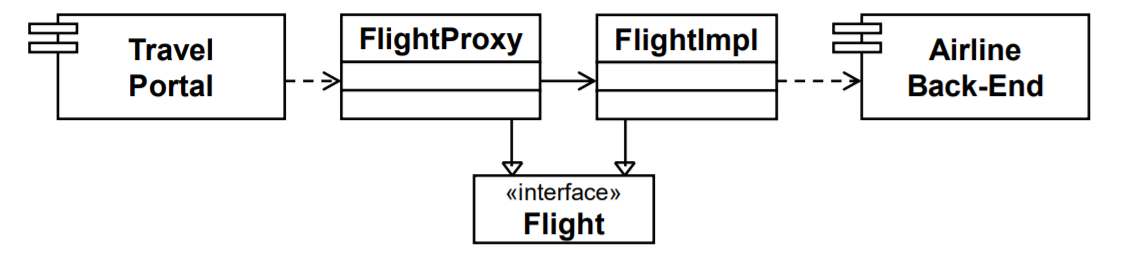
\includegraphics[scale=0.8]{mynd} \\
\section{Polymorphism}
Aðferðir sem eru yfirskrifaðar þannig að sama aðferðin er hægt að nota fyrir marga hluti.










\end{document}